% #############################################################################
% This is Chapter 4
% !TEX root = ../main.tex
% #############################################################################
% Change the Name of the Chapter i the following line
\fancychapter{Results}
%%%%%%%%%%%%%%%%%%%%%%%%%%%%%%%%%%%%%%%%%%%%%%%%%%%%%%%%%%%%%%%%%%%%%%%%
%                                                                      %
%     File: Thesis_Results.tex                                         %
%     Tex Master: Thesis.tex                                           %
%                                                                      %
%     Author: Francisco Azeredo                                        %
%     Last modified :  2 Jul 2015                                      %
%                                                                      %
%%%%%%%%%%%%%%%%%%%%%%%%%%%%%%%%%%%%%%%%%%%%%%%%%%%%%%%%%%%%%%%%%%%%%%%%
\label{chapter:Results}

\section{Information extraction and Structuring}
Some more complex multimodal models were tested in the beginning of the thesis for better information extraction.
\begin{itemize}
    \item \textbf{PrimaLayout}: Identifying and classifying regions such as text, tables, and images.
    \item \textbf{PubLayNet}: Segmenting documents into logical blocks.
    \item \textbf{Nougat}: An OCR engine that converts documents into markdown, preserving the hierarchy of chapters, sections, and subsections.
\end{itemize}
With testing, PrimaLayout, and PubLayNet promise good results with good training. This models unfortunately are not well trained yet, and need to be refined, as results were very unpredictable. Nougat was the engine used in case the pdf document doesn't have a text metadata.

\section{Experiment with metadata extraction versus naive RAG}
In this setup, answers were generated by our RAG system, which employed a sentence embedding model \textit{all-MiniLM-L6-v2} for retrieval embeddings and a local \glsxtrfull{LLM}, \textit{Qwen2M}, for generation in the offline benchmark. 
Each generated answer was then compared against its gold reference using the evaluation metrics reported below. 
These experiments relied on local models to provide a cost-effective baseline; stronger results were observed with larger hosted models but were too expensive to run this benchmark.

The experiment compares knowledge-graph–aware retrieval (Mini and Light) against a naive baseline.
Figure~\ref{fig:Lihua-World} presents the results across all metrics.
\begin{figure}[H]
    \centering
    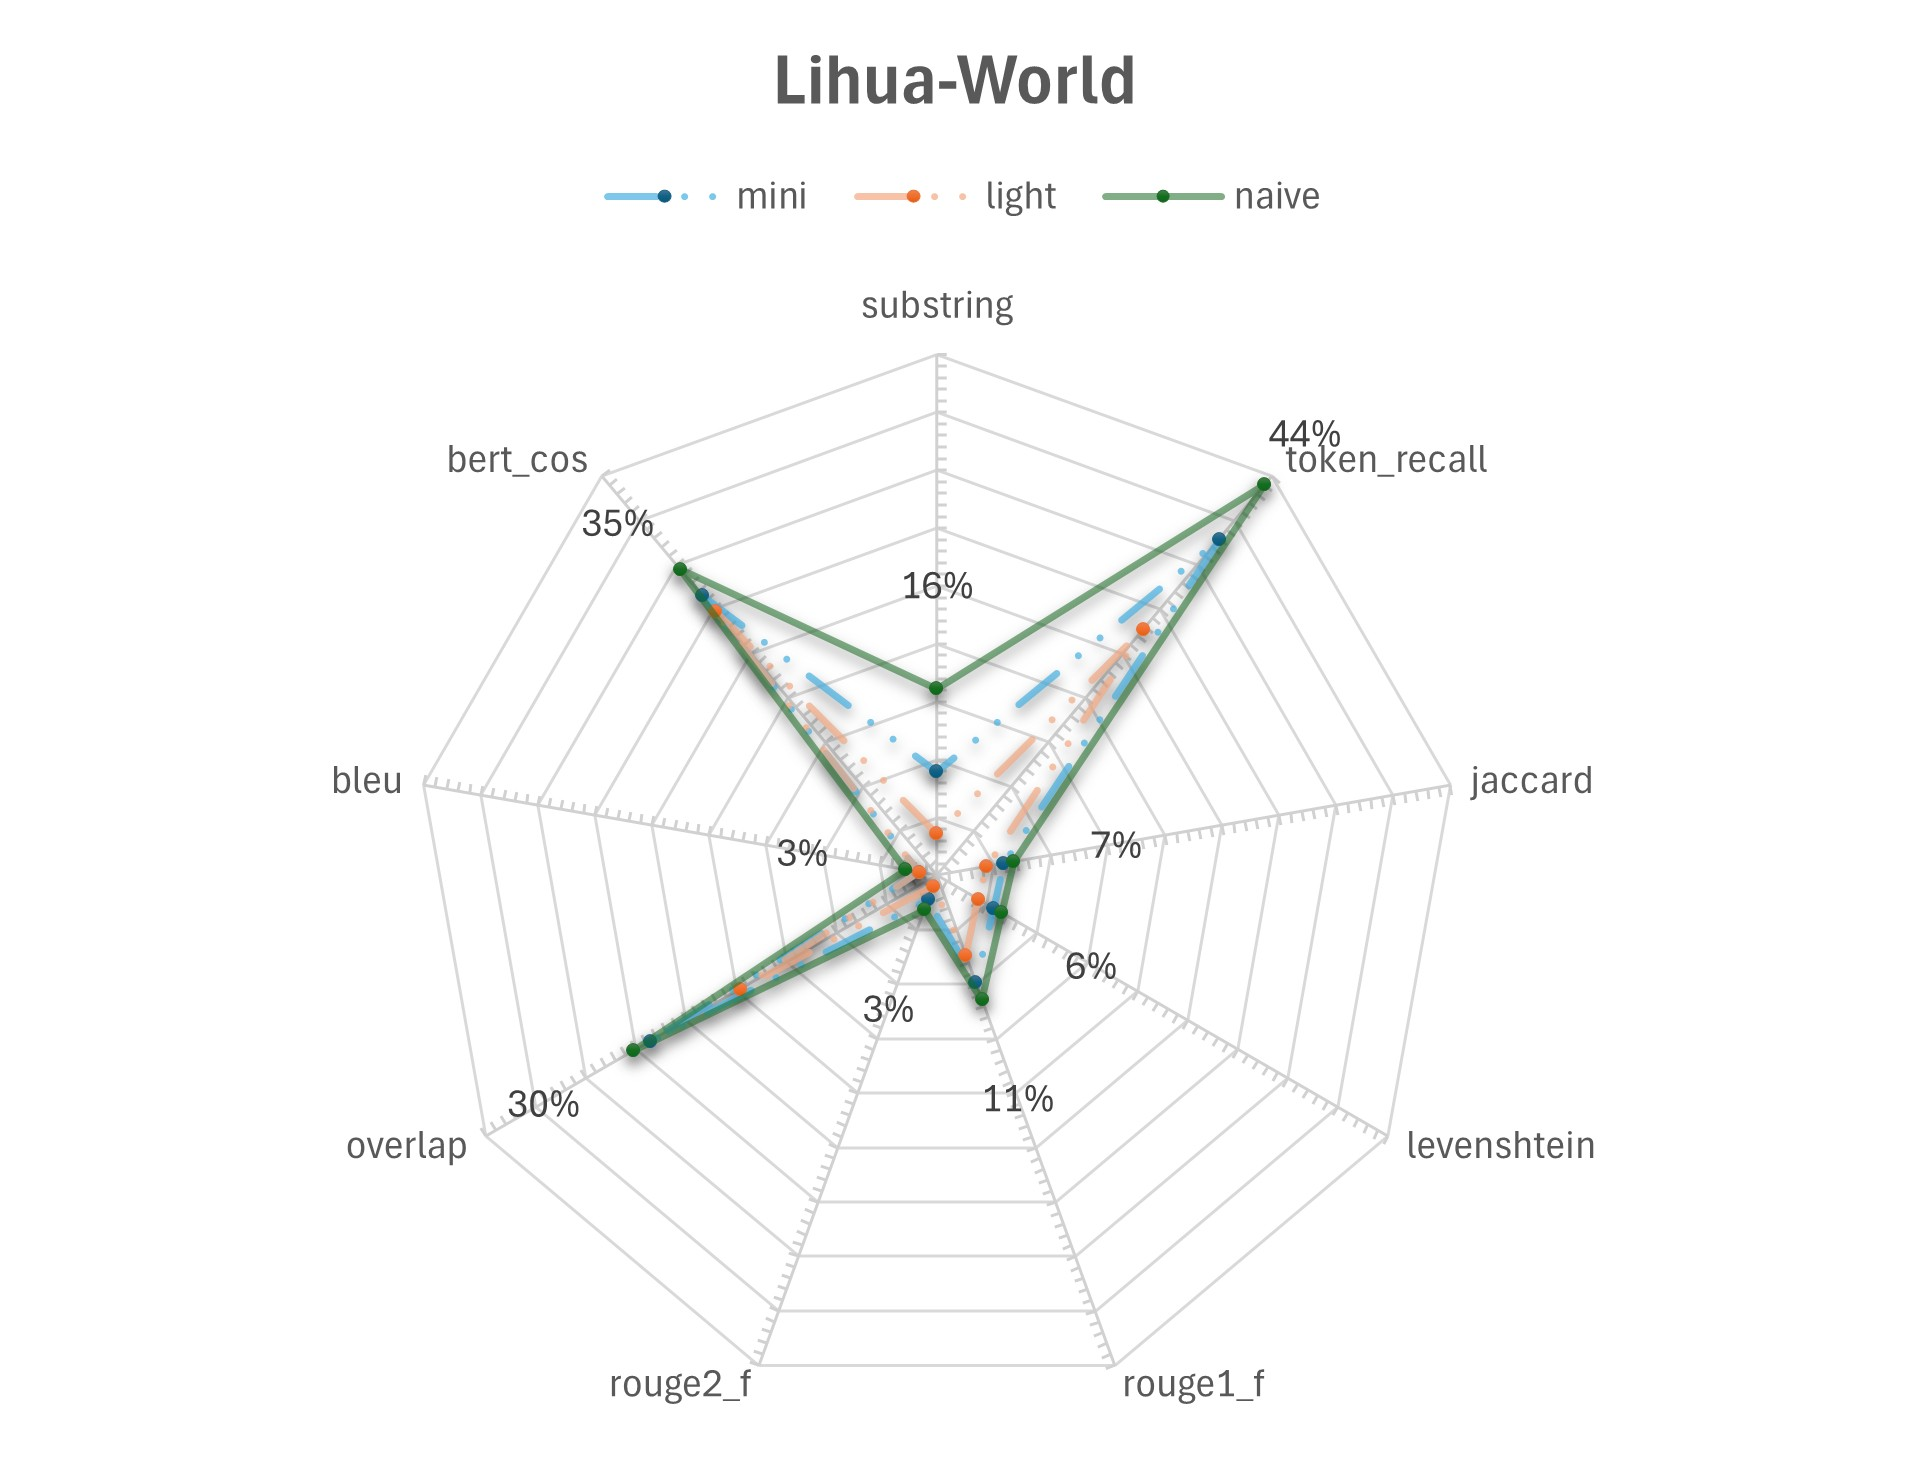
\includegraphics[width=1\linewidth]{Figures/Lihua-World.jpg}
    \caption{3 query types tested. With qwen2m as the llm and all-MiniLM-L6-v2 as embedding model}
    \label{fig:Lihua-World}
\end{figure}
Among the metrics, \textbf{Token Recall} achieved the highest score (44\%), confirming its relevance as a benchmark measure, since it directly evaluates whether the essential tokens of the gold answer are covered in the prediction. 

\subsection{Semantic Equivalence} 
\textbf{BERT cosine similarity} obtained a moderate score (35\%), typically remaining around 0.3 even when the correct answer was present. 
This can be explained by the imbalance between very short gold answers (sometimes a single word) and longer generated responses. 
Sentence-level embeddings such as \textit{all-MiniLM-L6-v2} capture global semantics, so comparing a single-token embedding with a full-sentence embedding often results in artificially low similarity scores.

\subsection{Lexical Accuracy} 
\textbf{Token Recall} achieved the highest score (44\%), confirming its relevance as a benchmark measure, since it directly evaluates whether the essential tokens of the gold answer are covered in the prediction. 
The \textbf{Overlap Coefficient} also scored relatively well (30\%), as it only checks whether the gold answer is contained within the generated text, without penalizing additional tokens. 
This makes it more robust than Jaccard in cases with large length differences between gold and predicted answers.

\textbf{Jaccard similarity} (7\%) produced very low values, since gold answers were often short while generated answers were longer, inflating the union size and reducing the overlap proportion. 
This means that even partially correct answers were scored poorly when extra words were present.

\subsection{Structural Similarity} 
\textbf{Levenshtein similarity} (6\%) also failed to provide useful signals, as the edit distance was large when comparing short references to long generated texts.  
\textbf{ROUGE-1 F1} (11\%) and \textbf{ROUGE-2 F1} (3\%) partially mitigated this by accounting for both recall and precision over n-grams. 
However, scores remained low because generated answers frequently included irrelevant tokens, which reduced precision despite containing the correct content. 
The ROUGE-2 score was particularly low because short gold answers rarely contained bigrams, making exact matches uncommon.  
Finally, \textbf{BLEU} performed worst (3\%). 
Originally developed for machine translation, BLEU is highly sensitive to exact n-gram matches and brevity penalties, which makes it unsuitable for this task given the mismatch between short references and longer generated predictions.

\subsection{Summary}
The experiments further show that GraphRAG is computationally too heavy for the modest gains it provides. 
Even its optimized variants, LightRAG and MiniRAG, remain relatively expensive and yielded weaker results compared to a direct sentence embedding retriever, which is both cheaper and more efficient. 
With stronger embedding models, this efficiency gap only widens, reinforcing the conclusion that knowledge-graph–based retrieval is not the most effective method for making a reliable and scalable search engine. 
Instead, a more promising direction is \emph{Agentic RAG}, explored later in this work, where retrieval is guided dynamically by agent reasoning rather than static graph structures.

\section{Experiment: Naive vs.\ Agentic RAG with Company Information}

For this experiment, a set of 20 questions was constructed using a generative model (specify model). Each question was designed to be answerable only through the content of a specific company file, ensuring that success required both correct retrieval and grounded reasoning.  

The baseline (naive RAG) simply retrieved top-ranked passages and generated an answer from them.
Then a CoT template was used on top of the baseline naive RAG.
In contrast, the agentic setup employed RAG with an MCP Weaviate server as the retrieval backend. The agent explicitly planned its approach before answering, dividing the task into structured steps:  
\begin{enumerate}
  \item Identify candidate documents by querying the Weaviate server for relevant information.  
  \item Select the file most likely to contain the correct answer.  
  \item Use the selected file as grounded context to generate a concise, final answer.  
\end{enumerate}

This setup highlights the difference between direct retrieval and generation versus a planning-based agentic approach that reasons over retrieved context.
\subsection{Naive RAG results}
% --- Lexical Accuracy ---
\begin{table}[h]
\centering
\begin{tabular}{lccc}
\hline
 & Token Recall & Jaccard & Overlap \\
\hline
\textbf{Correct} & 94\%\,(0,0\%) & 59\%\,(0,3\%) & 87\%\,(0,8\%) \\
\textbf{Wrong}   & 51\%\,(4,9\%) & 22\%\,(1,2\%) & 51\%\,(4,3\%) \\
\textbf{Total}   & 55\%\,(6,1\%) & 26\%\,(2,4\%) & 55\%\,(5,1\%) \\
\hline
\end{tabular}
\caption{Lexical accuracy metrics. Variance shown in parentheses.}
\end{table}


% --- Structural Similarity ---
\begin{table}[h]
\centering
\begin{tabular}{lcccc}
\hline
 & Levenshtein & ROUGE & ROUGE 2 & BLEU \\
\hline
\textbf{Correct} & 58\%\,(0,0\%) & 73\%\,(0,1\%) & 63\%\,(0,5\%) & 51\%\,(0,2\%) \\
\textbf{Wrong}   & 17\%\,(1,8\%) & 33\%\,(2,2\%) & 18\%\,(2,6\%) & 11\%\,(1,5\%) \\
\textbf{Total}   & 21\%\,(3,2\%) & 38\%\,(3,5\%) & 23\%\,(4,3\%) & 15\%\,(2,8\%) \\
\hline
\end{tabular}
\caption{Structural similarity metrics. Variance shown in parentheses.}
\end{table}

% --- Semantic Equivalence ---
\begin{table}[h]
\centering
\begin{tabular}{lc}
\hline
 & BERT Cosine \\
\hline
\textbf{Correct} & 82\%\,(1,4\%) \\
\textbf{Wrong}   & 72\%\,(0,4\%) \\
\textbf{Total}   & 73\%\,(0,6\%) \\
\hline
\end{tabular}
\caption{Semantic equivalence metric. Variance shown in parentheses.}
\end{table}

\subsection{CoT RAG results}
Have results but still thinking how to put them
\subsection{Agentic RAG}
Have results but still thinking how to put them

%\begin{figure}[h!]
%    \centering
%    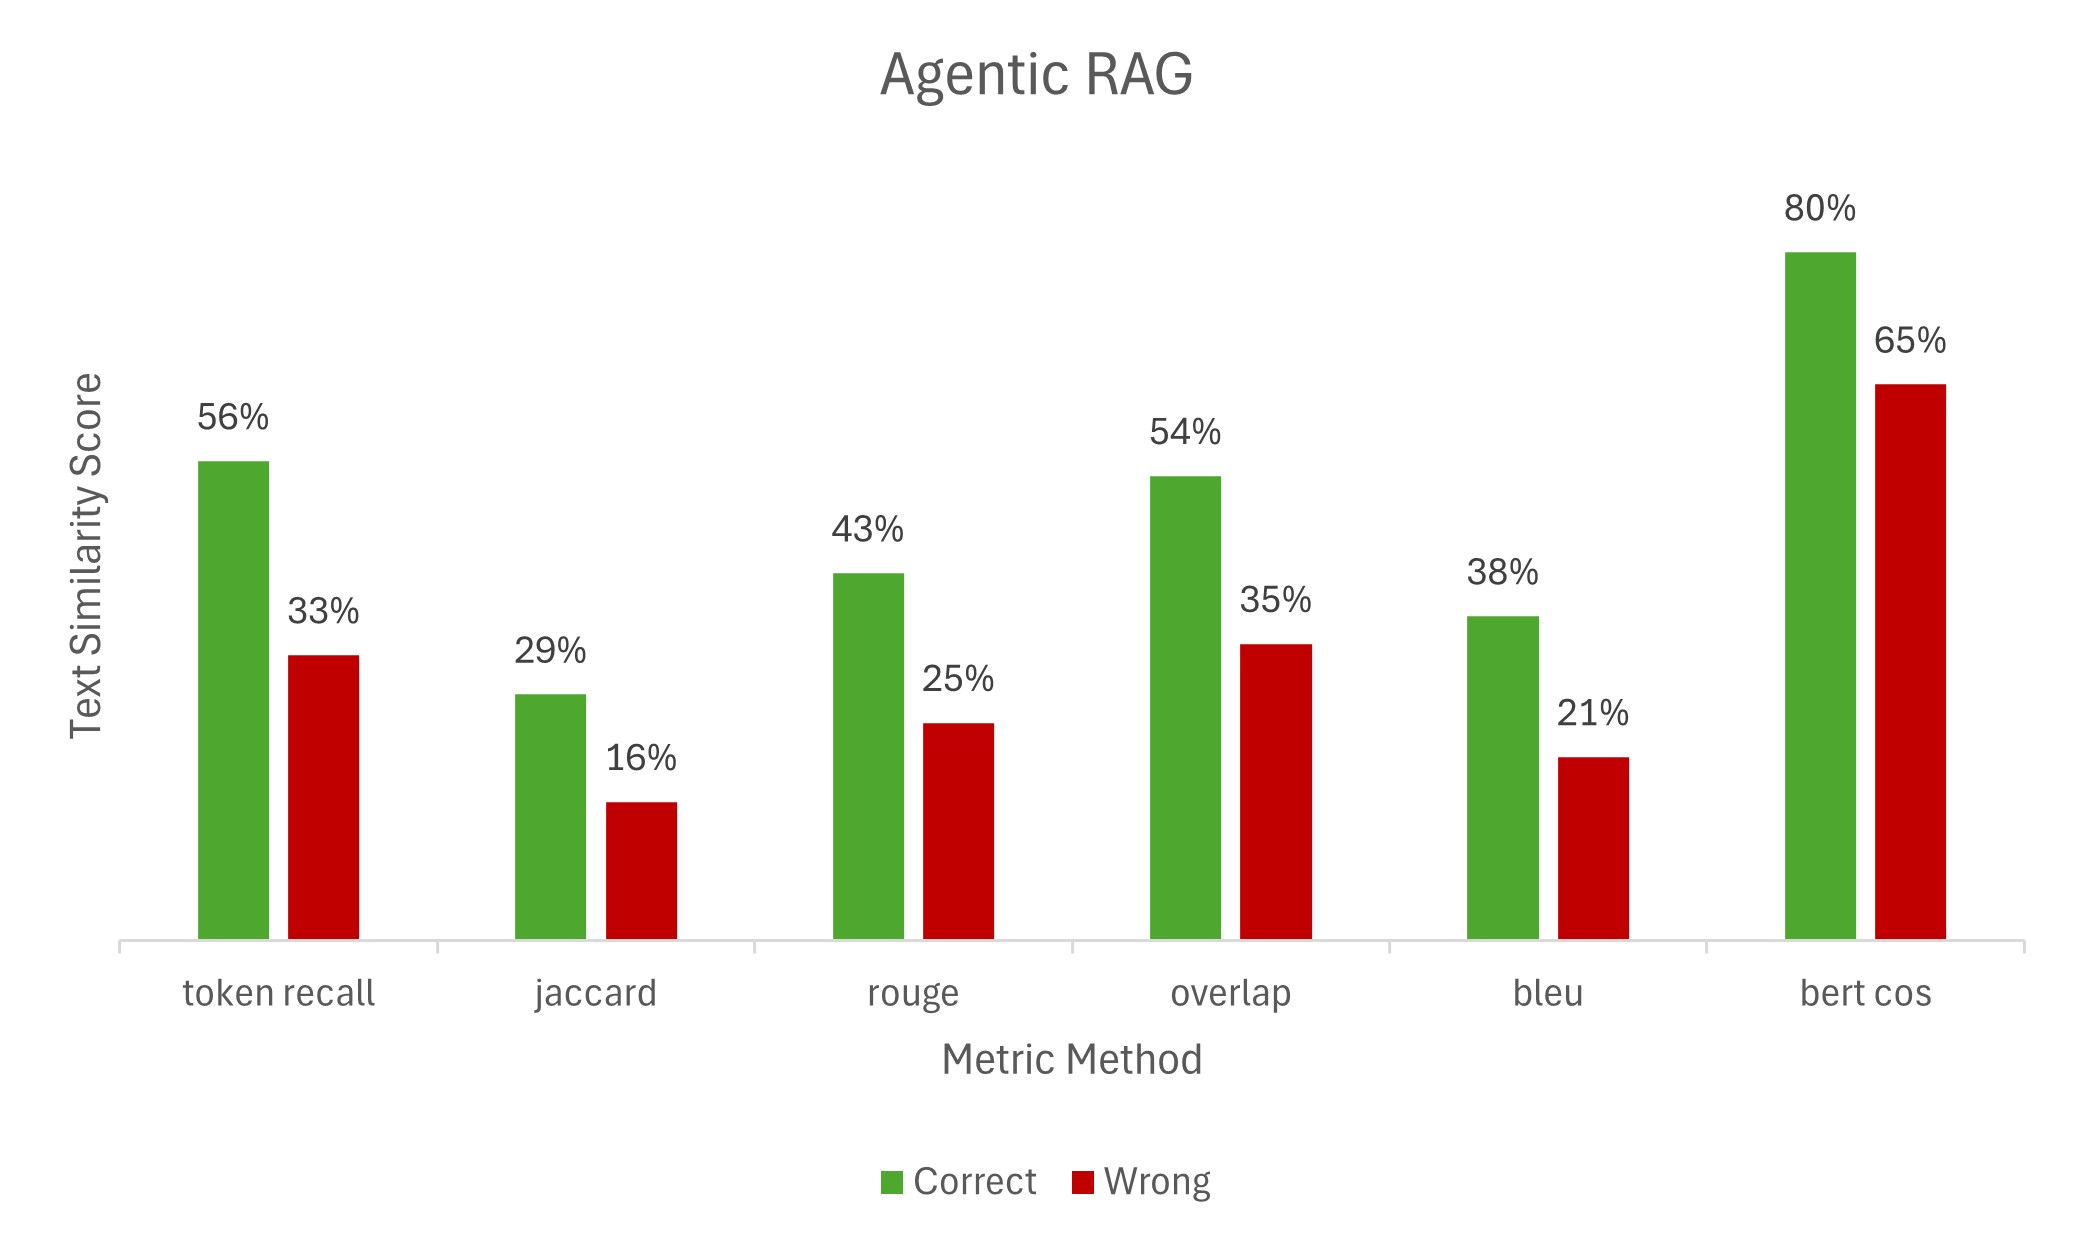
\includegraphics[width=0.75\linewidth]{Figures/Agentic_Semantic_Score_Hallucination.png}
%    \caption{Agentic Semantic Score, with chatgpt5-mini}
%    \label{fig:placeholder}
%\end{figure}
%
%\begin{figure}[h!]
%    \centering
%    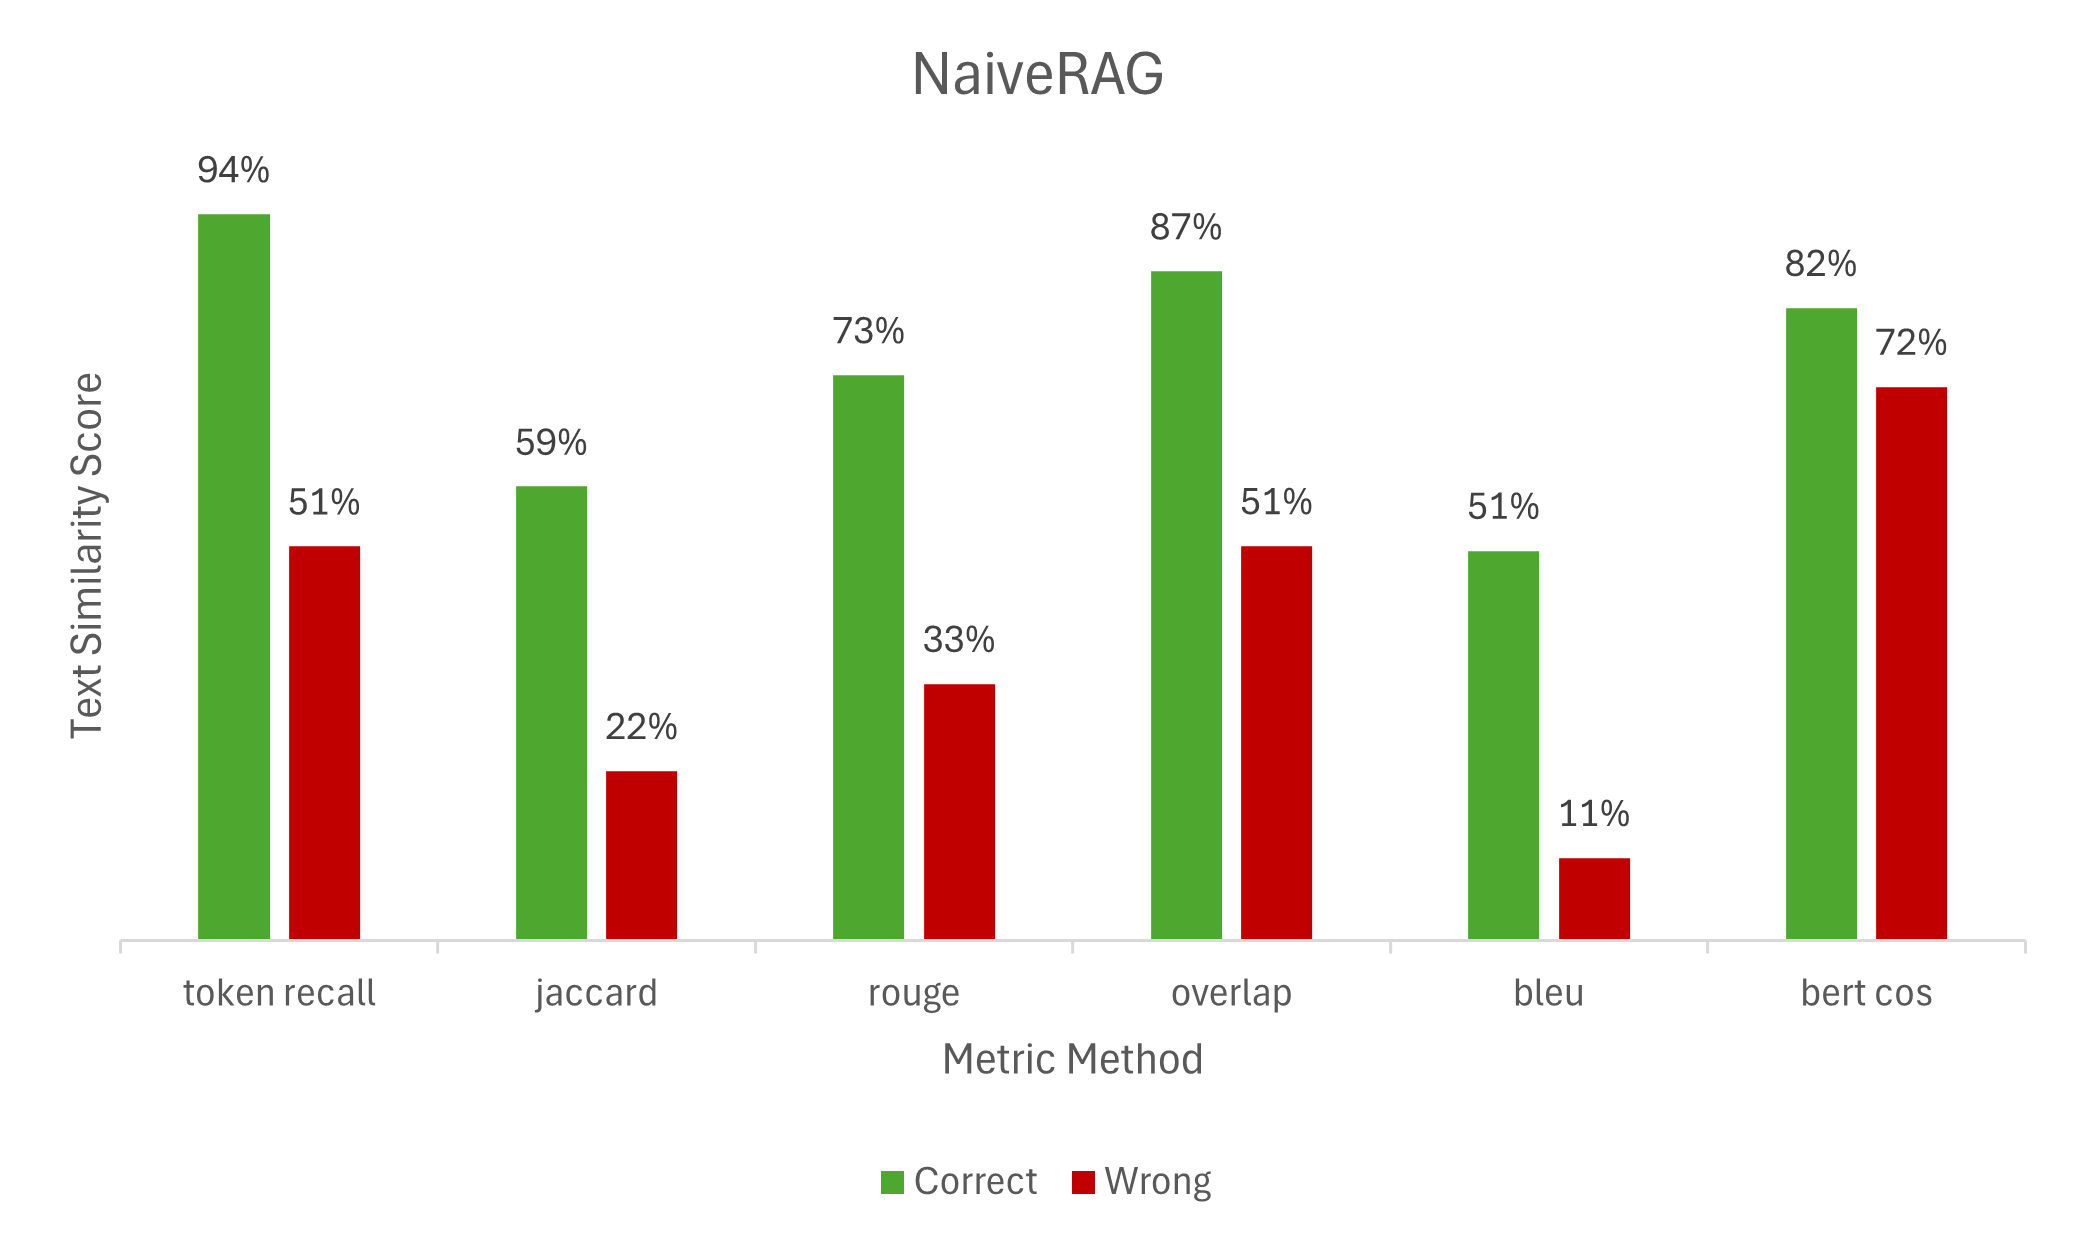
\includegraphics[width=0.75\linewidth]{NaiveRAG.png}
%    \caption{With Qwen2.5m}
%    \label{fig:placeholder}
%\end{figure}

%\begin{figure}
%    \centering
%    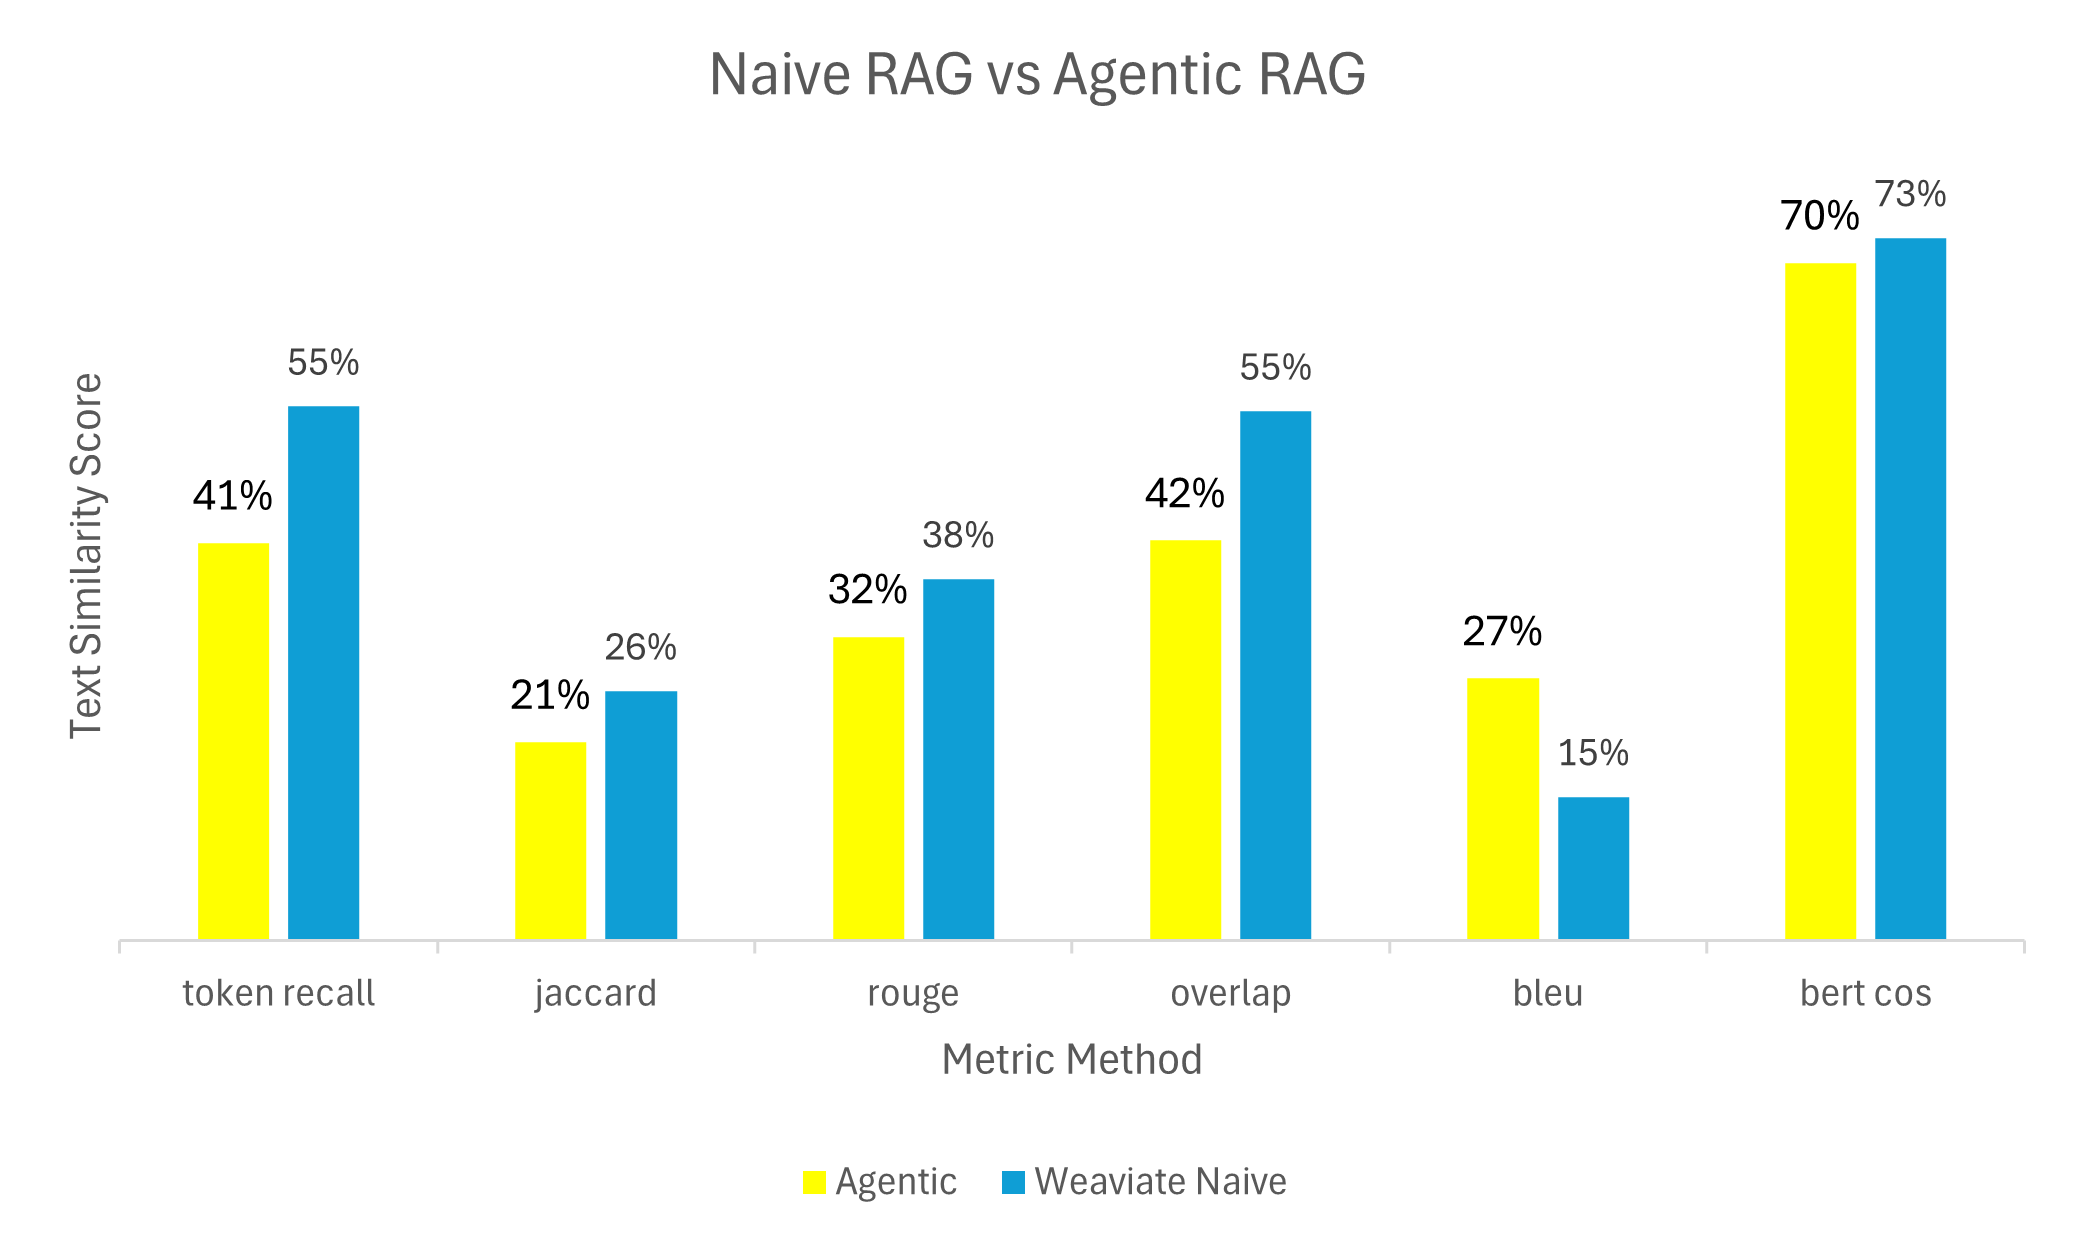
\includegraphics[width=0.75\linewidth]{Naive Rag vs Agentic Rag.png}
%    \caption{Total}
%    \label{fig:placeholder}
%\end{figure}

\subsection{Overall Results}
\begin{figure}
    \centering
    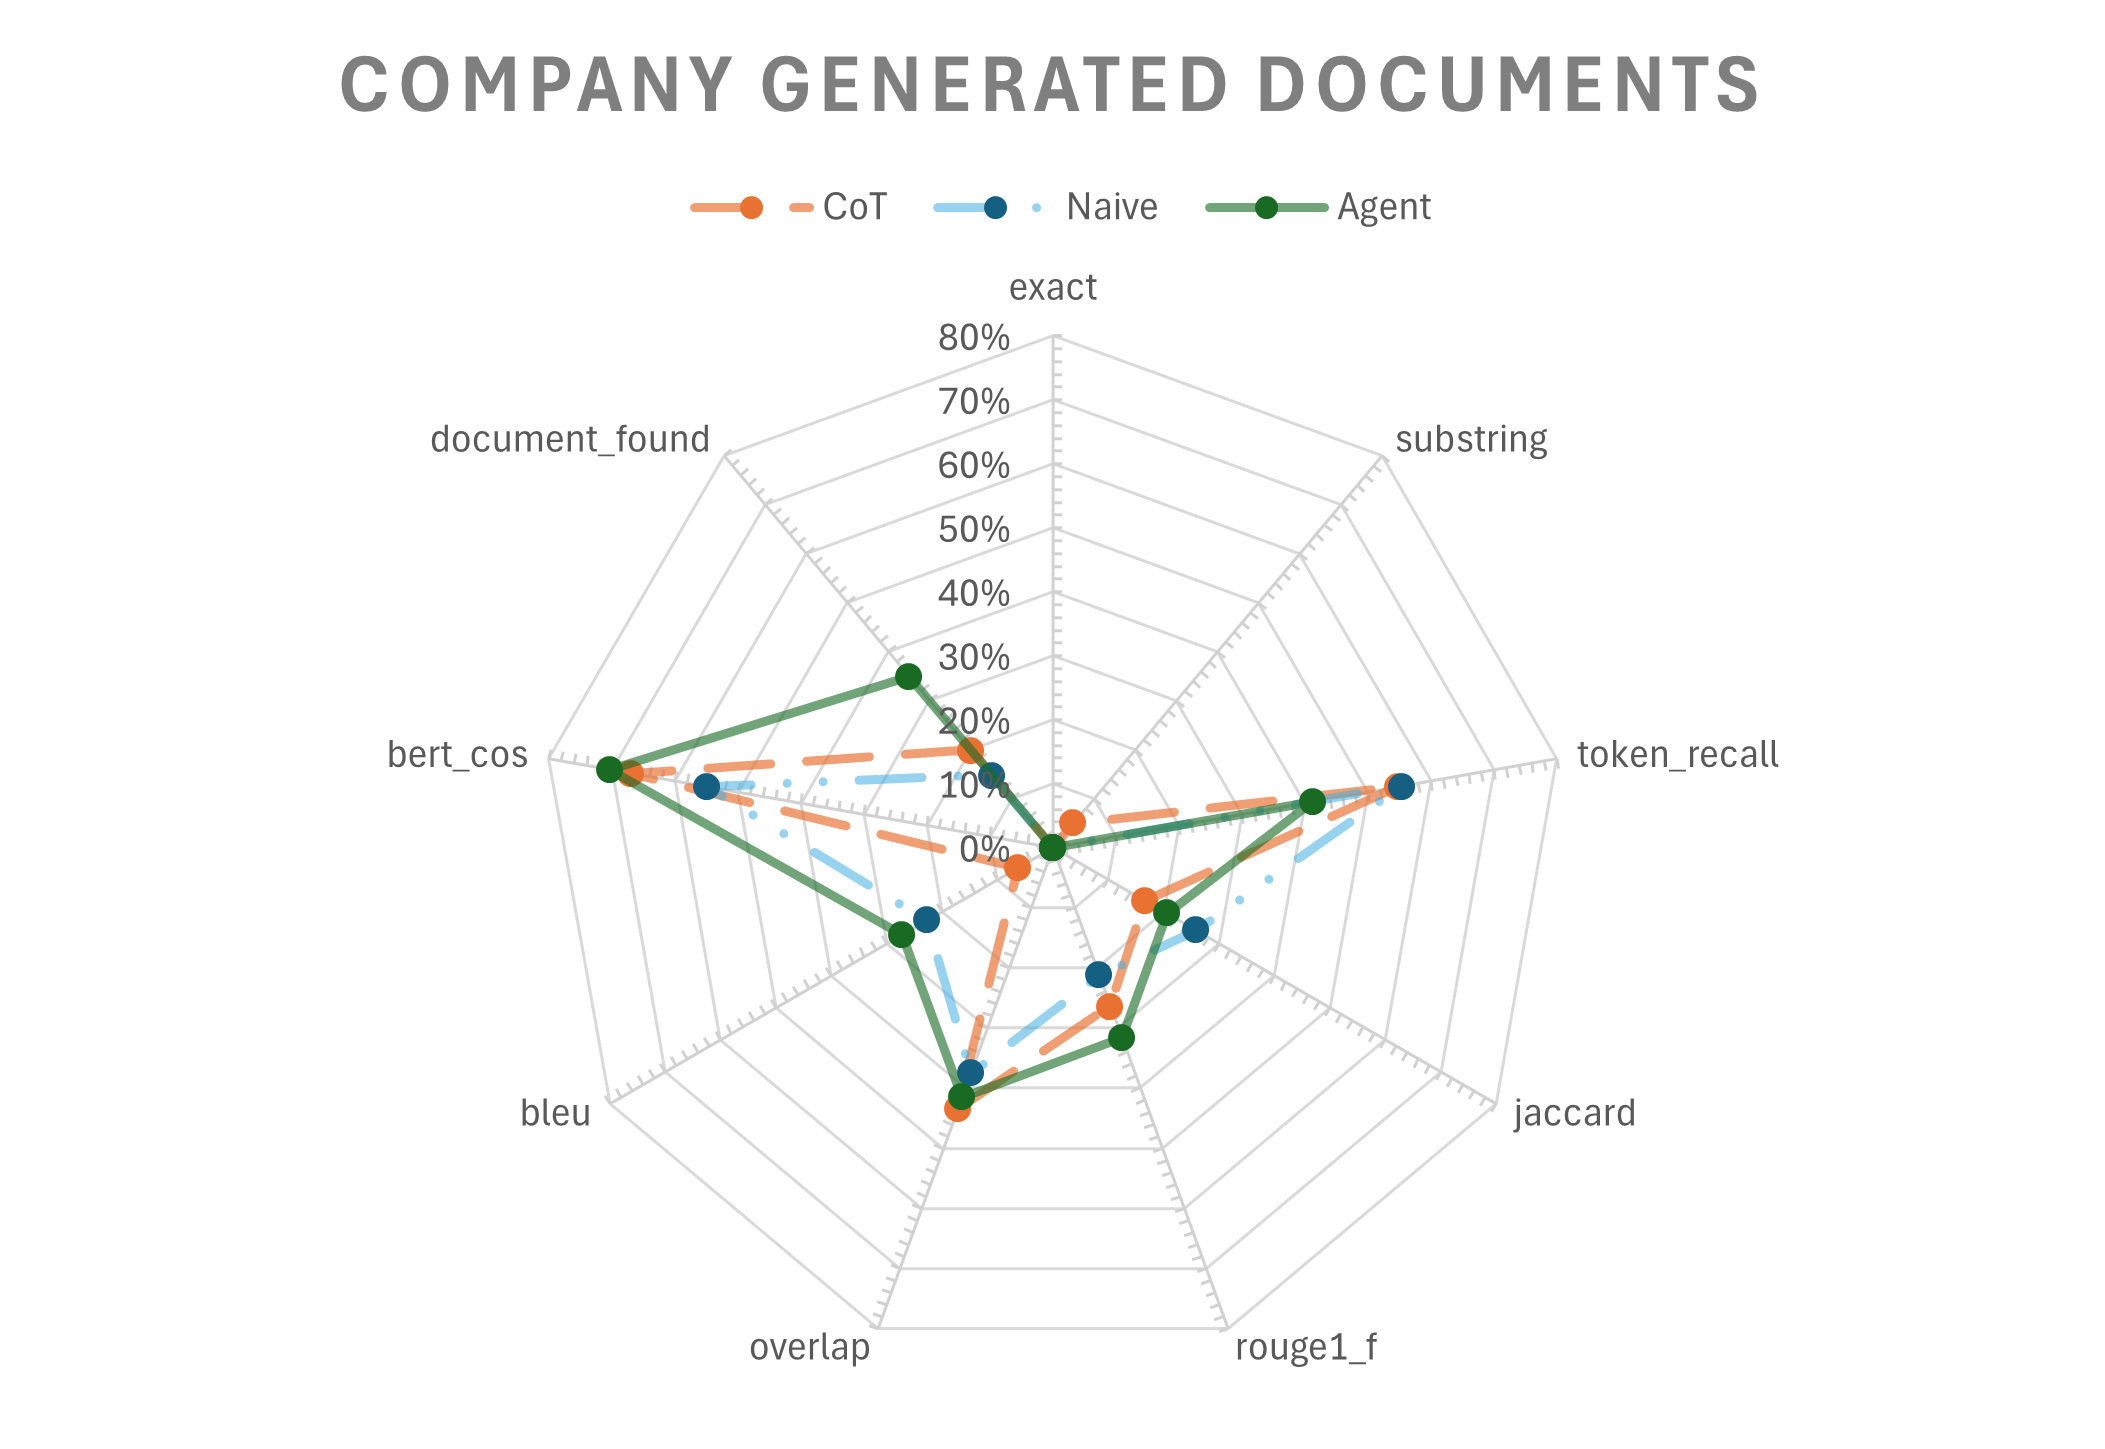
\includegraphics[width=1\linewidth]{Figures/Company Generated Documents.png}
    \caption{Enter Caption}
    \label{fig:placeholder}
\end{figure}





